Designing easily extensible and testable numerical codes is inherently challenging,
the complexity of numerical algorithms and the continuous nature of their results
make it hard to separate the logic from application specific implementation details.
As \gls{PyExaFMM} is implemented in Python, an \gls{interpreted} and inherently
\gls{object-oriented-language}, we are able to
use some common and powerful object oriented design principles to ensure extensibility
and testability. However, as most parallel optimisation software relies on access to data
containers themselves, rather than an abstraction layer between a data object
and a client object, the number of object abstractions must also be kept to a
minimum.

Concerns about the overhead of using the object oriented design principles, in comparison to directly manipulating
primitives, such as those available in lower level compiled languages such as C
or C++, are misplaced for two reasons. Firstly, the implementation of Python objects
is syntactic sugar, methods and data for a given object are written into
a simple dictionary structure at run time, with the `class' syntax common to other
object oriented languages such as C++ or Java, offered as they are familiar to
the programmer coming from such languages. Resultantly, all `primitives' such as
integers and strings in Python are actually objects by design, being quite different
in their construction from C or C++ where the programmer is given the power to
allocate memory for true primitives themselves. In Python the overhead therefore
comes from the interpreter, which transforms the source code into byte code which
is then compiled. This additional interpreter layer is the source of Pythonic overhead,
rather than the object abstraction in itself. Therefore, once the decision has
been made to use Python, there isn't a significant overhead from using object
oriented design principles, with the added benefit of increasing programmer
productivity, and increasing testability \cite{Ramalho:2015:Oreilly}. Secondly,
the vast Python ecosystem of optimised libraries for numerical computation allow
for the manipulation and allocation of primitives in memory in a manner closer to a compiled language.
Specifically, \gls{PyExaFMM} implements all of its containers with NumPy, which
offers an interface for the allocation and access of numerical data with C-like
efficiency, due to the underlying subroutines being written in C. Additionally,
\gls{PyExaFMM} uses just-in-time (\gls{JIT}) via the Numba library on
numeric subroutines implemented with NumPy containers. Just-in-time compilation
refers to a system which analyses the byte-code of generated by an interpreter
for repetitive operations which would benefit from compilation and caching, therefore
combining the speed benefits of compiled languages, with the flexibility of interpreted
languages.

\begin{figure}
    \centering
    {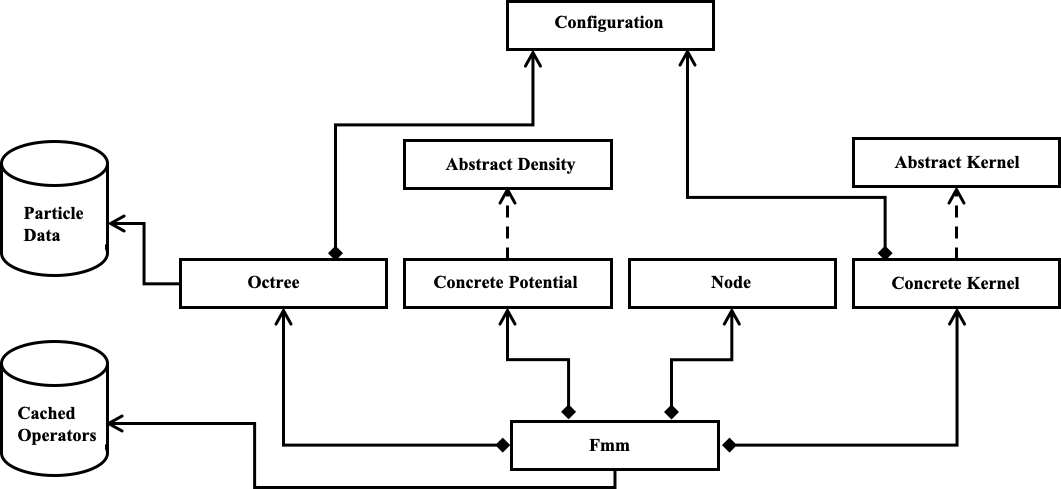
\includegraphics[width=\textwidth]{chapter2/object_organisation.png}}
    \vspace{0pt}
    \caption{Object hierarchy of \gls{PyExaFMM}. Objects are illustrated with
    square boxes, and data (either on disk, or in a cache) by a cylinder using
    standard software engineering convention \cite{Gamma:1994:Addison}. Solid
    lines indicate a dependent relationship, whereas the dashed equivalent
    indicate an inheritance relationship. A diamond arrow head indicates an
    object instantiation, a pointed arrow head indicates the direction of a
    dependency.}
    \label{fig:2_5_architecture}
\end{figure}

\begin{figure}
    \centering
    {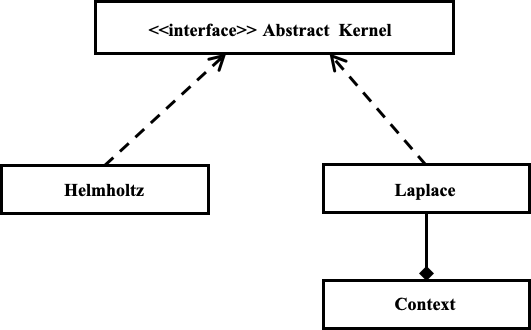
\includegraphics[width=0.6\textwidth]{chapter2/kernel_strategy.png}}
    \vspace{0pt}
    \caption{Strategy design pattern implemented for the Kernel class.  Solid
    lines indicate a dependent, relationship the dashed equivalent
    indicate an inheritance relationship. A diamond arrow head indicates an
    object instantiation, a pointed arrow head indicates the direction of a
    dependency.}
    \label{fig:2_5_strategy_kernel}
\end{figure}

The main object hierarchy used in \gls{PyExaFMM} is shown in figure
(\ref{fig:2_5_architecture}). The first major design principle followed is dependency
inversion, whereby components are arranged in a hierarchy such that downstream
modules are not dependent on upstream modules for any of their logic, and coupled
to them via abstractions \cite{Gamma:1994:Addison}. \gls{PyExaFMM} is architected
around the main `Fmm' object, which is placed at the top of the object hierarchy.
This object contains methods for running the upward and downward pass steps of the
\gls{FMM} loop, as well as access methods for the source and target particle data,
and the results of the expansion at each level of an associated octree. In \gls{PyExaFMM}, a configuration
object, specified via a \textbf{\gls{JSON}} configuration file, is instantiated
at runtime. This is resultantly used to instantiate an Fmm object, from the bottom
up, with its dependencies. Namely, an Octree object is configured, which instantiates
a linear octree as well \gls{JIT}'ing associated bitwise methods for tree traversal, from
user specified source and target particle data - the locations of which on disk are
specified by the configuration file. Additionally, a user specified kernel function
configures a kernel object. This kernel object is defined using the strategy design pattern
\cite{Gamma:1994:Addison}, illustrated in figure (\ref{fig:2_5_strategy_kernel}).
This pattern allows for concrete implementations of kernel objects to be separated
from the context in which they're used, allowing the user - in this case the
Fmm object - to access kernel functions via a uniform interface. Kernel
objects, in addition to the kernel function, allow for the encapsulation of
kernel specific information such as their scaling properties at different levels
of an octree. The configuration file further specifies the specifics of a simulation; such as the order the
multipole and local expansions, and parameters to take for the relative size of
the check and equivalent surfaces as well as the SVD compression tolerance for the
M2L operator matrices. However the main point to note is that a loose hierarchy
of objects allow for the logic of the main \gls{FMM} loop to be separated from
the creation and partitioning of an octree, including the code required for
its traversal, as well as the implementation specifics of a simulation, such
as the kernel function used, and parameters for surface creation and the SVD.
Safety is further enforced by interfaces for data, specifically the Abstract
Density and Node classes define interfaces for access to concrete Charge/Potential density
objects and octree nodes respectively, as well as their underlying Numpy based containers,
in a uniform manner. These types of objects, often referred to as return objects
as they specify the format of a computation being returned, are a common trope in
object-oriented design, and help enforce an expected client
interface, as the main Fmm object is able to rely on guaranteed container
datatypes and data dimensions enforced by the return objects.

The second major design principle followed by \gls{PyExaFMM} is
the separation of concerns, whereby implementation details of distinct
components of a program are separated by modules, with known interfaces
\cite{Gamma:1994:Addison}. Specifically, \gls{PyExaFMM} separates into scripts
the code for operator caching discussed in Section \ref{sec:2_3_operator_caching},
and the code for SVD based compression of the M2L operator matrices discussed in
Section \ref{sec:2_4_svd_compression}. These scripts are accessible via the
command-line, through a custom command-line interface, invoked with the command
prefix `ci', created as a part of \gls{PyExaFMM} package. We refer to the \gls{PyExaFMM} documentation for more information,
however a basic workflow would start at the command line, creating and compressing
the operator matrices

\begin{verbatim}
Last login: <Day> <Month> <Date> 00:00:00 on console
user@Workstation ~ % ci compute-operators
user@Workstation ~ % ci compress-m2l
\end{verbatim}

These commands are again configured using the \gls{JSON} configuration file.
Following them, \gls{PyExaFMM} is automatically configured with the required
operator and particle data, and simulations can be run from within a Python
interpreter or as a script using the following framework,

\begin{python}
from fmm.fmm import Fmm

# Instantiate FMM object
fmm = Fmm(config_filename='my_custom_config.json')

# Run Upward Pass
fmm.upward_pass()

# Run Downward Pass
fmm.downward_pass()

# Get Results at Target Points
fmm.result_data
\end{python}

At runtime, the instantiation of the Fmm object is preceded by the injection of
dependencies from beneath it in the object hierarchy. However, this complexity is
easily hidden from the user, who only specifies simulation parameters and source
and target particle data locations via a \gls{JSON} configuration file.
